\setlength{\footskip}{8mm}

\chapter{Literature Review}
\label{ch:literature-review}

Text detection and recognition most commonly referred to as OCR(Optical Character Recognition) is an actively participating area in the research that uses deep learning methods as state-of-art and keeps evolving with the improvements in deep learning models. \cite{history} OCR is considered a prerequisite step for the conversion of image-based documents to digital structured digital text. This is because when we input any image or video-based (unstructured) data to any machine learning model it needs to be preprocessed before and OCR is indeed preprocessing step. \cite{real-world} Text detection and recognition is not an easy task therefore primitive machine learning methods can not help to achieve high accuracy. But with the advancement in deep learning techniques, we are now able to get promising results.
If we explain OCR in one line OCR is information transfer from the image domain to the text domain. This information transmission comprises two steps first is the detection and the second is recognition.

\section{Text Detection}
In detection, we find optical characters in a given image. Primitive OCR models assume fixed templates in images for example text detection from pdf documents. But in the case of natural scene images template of images may vary depending upon various factors like light intensity, scaling, shape, orientation, etc. If we compare text detection from documents and natural scenes here we see natural scene images text detection has some other unique challenges. \cite{deep_learning_era} As compared to documents, text in natural scenes experiences variability and diversity. In natural scenes, text may be from different languages and may face geometric effects like different font sizes and font styles. Orientations, shapes, and colours may also differ. Besides this, scene texts may pose different aspect ratios and layouts. Secondly, Natural scene images may face abnormalities in the background like background texture may differ from image to image because natural scene images may have diverse scenery. Background can have pattern which is exact match of text so it can lead to confusion and mistakes. Thirdly, images may have been taken in uncontrolled circumstances where they can face photometry effects like illumination, brightness, and resolution issues. In an environment where we have poor light images will have a low resolution so the image may be corrupted because of shadows and highlights. Shooting distance may also affect the quality of images and it can lead to the scale space problem. If a camera is shaken while taking an image it may blur the image and may introduce noise in it. Here we need an efficient and robust approach to character detection. This led to the invention of the convolutional neural network(CNN) considered a most powerful tool for feature map extraction. CNN gives us many CNN-based object detection models like R-CNN, SSD and FCN etc. %There are again improved versions of all these models like fast and faster R-CNN. 


\subsection{Classical Methods}
Before the rise of deep learning hand crafted features were in practice for text detection. In literature, we can see many methods for separating text strings from images. All are listed below.
\begin{enumerate}
    \item \textbf{Text and non-text separation Method} \newline
    Text and non-text separation \cite{offline} is a type of method in which text strings and graphics are separated in a way:
    
    Suppose I is a set of images and $ \in $ is the set of output 
    \begin{equation}
    \label{eqn:Text and non-text separation Method}
    \in = \{ CT , CNT \}
    \end{equation}
    where CT represents text-class and CNT represents non-text Class

     Text non-text separation method started in 1980 authors \cite{matching} developed combined symbol matching (CSM) system where they recognized characters by assigning certain ASCII codes. This system was sensitive to character font size and font style. For every change in font style and font size change system has to run once with different parameters. \cite{block-segmentation} algorithms were designed to classify text and graphics regions. \cite{gray-level} In 1984, the author proposed a method for extracting lines from grey-scale images of industrial design. Here algorithm is document specific too which only processes grey-scale images. \cite{electrical-segmentation} This paper used segmentation to divide electrical schematics into primary components. But this algorithm is also sensitive to changes in text size and font style. As this algorithm breaks components into sub-components so graphic recognition becomes a difficult task. Many other other authors also tried to apply this method and text/non text separation method keeps improving in preceding years \cite{robust-1999} \cite{text-finder} \cite{text-in-images}. 
    \item \textbf{Texture Based Methods} \newline
      Texture-based methods \cite{detection-advancements} are based on textual properties like local intensities, filter responses and wavelet coefficients. Here text is considered a special texture and these properties are used to separate text and non-text regions in images. These methods are computationally expensive because we need to scan all locations and scales here. Secondly, these methods only support horizontal texts and are sensitive to scale and rotational changes.
     \begin{enumerate}
        \item \textbf{Color-Segmentation}  
          In 1995, \cite{color-images} proposed text localization method from colored images.This method used horizontal spatial variance to find raw text and then located text regions on the basis of colour segmentation. After this text detection in videos was proposed by decomposing images via wavelet coefficients\cite{video-detection}. 
        \item \textbf{Machine Learning Classifiers}  
          Machine learning algorithms SVM(Support Vector Machine) and CAMSIFT(continuously adaptive mean shift algorithm) are robust for text detection from simple background images but this is sensitive to complex background \cite{CamSIFT}. Later \cite{video-svm} used pre-trained SVM to detect text from videos.Firstly used the Sobel filter to get features(edge map)and then fed it into SVM to get text/non-text regions. But this algorithm is different from conventional methods due to Discrete Cosine Transform(DCT) where there is no need to encode image before detection. It improved efficiency but decreases accuracy.
         \item \textbf{Adaboost Classifier based text-detector}  
           Researchers proposed fast detector \cite{fast-detector} which is cascade Adaboost \cite{adaboost-classifier} classifier in which weak classifiers combine to make strong classifier.Each weak classifier is trained on a features map. Feature map includes intensity variance, vertical differences, gradient, horizontal differences and means strength. Although, this detector is more efficient than other detectors in the past its accuracy is compromised on real-world images. Later \cite{unsupervised} proposed methodology based on unsupervised learning to learn features and develop a robust algorithm for both detection and recognition.
         
         \item \textbf{Sliding Windows}
         Sliding windows are used to locate specific words from natural scene images. \cite{text-in-wild} Used this method to detect texts in wild.In this method, firstly single character is detected then we match characters on the basis of structural relationships and finally most similar characters combination gives us the output. But this type of method can detect text on the basis of the given list. No text can be detected out of bound so this makes use of a detector limited to some narrow ranges as it is impossible to have a list of words for all images in the real world.
     \end{enumerate}
    
    \item \textbf{Component based methods} \newline
    This is a type of method in which candidate components are extracted through a number of ways like colour clustering or extreme region extraction etc. After features extraction, non-text regions are discarded with the help of classifiers or by manually designed rules which are automatically trained on hand-crafted features. Before deep learning components-based methods have been mainstream for scene text detection.
    
    Next, we have colour clustering method \cite{color-clustering} in which the image is decomposed into many non-overlapping components by colour clustering, by component, analysis components are grouped into text lines and non-text regions are removed as per geometric rules.As this system is trained on artificial parameters  and rules so shows poor accuracy on complex background images.
    
    Later \cite{SWT} made use of the characters property of having almost constant stroke width. On this basis proposed a new image operator called stroke width transform(SWT). By using this operator we can easily pick character strokes from the edge map and can easily extract characters of different orientations and scales. As this method also follows hand-crafted features it can only handle horizontal texts.
    
    There is another text detection \cite{MSER} algorithm using maximally stable extremal regions(MSER). Here MSER regions are considered as candidate regions of the image and eliminate invalid candidates using the classifier. And remaining candidates are grouped into text lines through connection rules. But this solution is only applicable to horizontal or nearly horizontal texts therefore this is sensitive to inclined angles. SWT\cite{SWT} and MSER \cite{MSER} are representative methods and these led to foundation of other subsequent works \cite{arbitrary}, \cite{real_time_detection}, \cite{stroke-n-co-variance}, \cite{conv-n-MSER}, \cite{edge-enhanced_MSER}, \cite{multi-oriented}.
    
    Sparse representation in face recognition \cite{sparse_face_recog} and image denoising \cite{img_denoising} opened ways for many other algorithms like \cite{sparse_detection} proposed algorithm to detect presence of text by building sparse dictionary of input images.But this algorithm is sensitive to rotation and scale changes.\cite{structure-based} Proposed solution to orientation problem by developing algorithm which can detect titled text.Later \cite{multi-oriented_text_in_videos} proposed solution to detect multi-oriented text in videos.
    On the basis of SWT \cite{arbitrary} proposed an algorithm to detect arbitrary shaped text in natural scene images. The speciality of this algorithm is a two-level classification, rotation and rotation-invariant features set designed to capture intrinsic features of characters in natural scene images.
    \cite{SFT} developed a new operator inspired by character width transform called stroke feature transform. Stroke width transform has mismatch problem of edge points so SFT provides colour consistency and constraints relations of local edge points which produces better extraction candidates. Detection results by SFT show better performance on standard datasets but are limited to horizontal texts.
    \item \textbf{Hybrid Methods}
    Hybrid methods make use of both texture-based and component-based methods. \cite{contour-based} made use of both component analysis efficiency and texture-based method robustness to detect text in colour images. First of all, an elaborate edge detection algorithm is applied to get all possible edge point points of the text. Then it's time to apply connected component analysis to extract internal and external contours to get potential candidate regions. There is a careful examination of geometric characteristics and gradient of the image to extract True text regions and finally, we classify  text or non-text regions.

    Later in 2019 \cite{hybrid} also get the benefit of the hybrid method. Here text detector is designed to get the confidence in text presence and this confidence level is scaled into an image pyramid which in turn helps in semantic segmentation to get text via local binarization. A conditional random field method(CRF) model is proposed to efficiently remove non-text components. At last, there is the use of energy-based learning minimization to get text lines/words from text components.
    
    Text awareness score can also be used to detect and localize text in natural scene images.\cite{text-awareness-score} authors proposed a novel text awareness approach which is based on a fast edge-preserving and smoothing Maximum Stable Extremal Region (FEPS-MSER) algorithm. This provides fast edge detection for text candidates.A naive Bayes classifier is used to find text and non-text regions.
\end{enumerate}

\subsection{Deep Learning Era}
\begin{enumerate}
    \item \textbf{Convolutional Neural Network(CNN)}  \newline
In earlier attempts to use deep learning researchers used a combination of deep and classical methods.\cite{CNN_MSER} combined Convolutional Neural Network(CNN) and Maximally Stable Extremal Regions (MSERs). MSERS can not deal with complex text information efficiently so it is not good algorithm to separate text from background. But CNN can effectively learn high-level features which help in robust text detection. This algorithm got 78\% F-measure which is higher than all classical and machine learning methods. \cite{arabic}made use of the convolutional neural network to detect text in videos. But in this method author solely made use of the deep learning model with no use of prior features extraction through hand-crafted methods. In 2008, \cite{CNN} uses CNN to text in a synthetic dataset but this method showed better performance on f ICDAR’03 real-time test data.\cite{text-flow} Developed text-flow with the use of convolutional neural networks to detect characters using a min-cost algorithm.
\cite{yao2016scene} used a convolutional neural network for pixel-level classification of text/non-text regions.This also has the capability to detect text orientation. After classification, all positive responses are grouped together and apply Delaunay triangulation algorithm\cite{Kang2014OrientationRT}. In the end, graph partition algorithms are applied which detect text lines on the basis of orientation attributes.\cite{FullyCNN} developed a novel methodology with the use of two fully convolutional neural networks. First FCN was trained to achieve salient maps of text regions holistically. Then we get text-line hypotheses with the combination of character components and feature map. Second FCN is trained as a classifier to classify the correct centroid of each character and remove false candidates. This algorithm proved to be state-of-the-art because of its performance on benchmark datasets: MSRA-TD500, ICDAR2015 and ICDAR2013. This algorithm is robust to multi orientations, languages and fonts. \cite{segmentation-CNN} spotted natural scene text in the wild where a multiscale fully convolutional neural network (FCN) is used to detect text regions. Then there is a novel instance (word or line) aware segmentation which removes false positives and finally gives true word instances. This algorithm is robust for detecting arbitrary oriented text and achieved state-of-the-art performance in ICDAR 2013 (IC13), ICDAR 2015 (IC15) and CUTE80 and Street View Text (SVT) benchmark datasets.
\end{enumerate}

\subsection{Methods Inspired by Object detection}
Text is considered a special kind of text so object detection techniques can also be implemented for text detection. However, text poses some unique challenges different from general object detection.

\begin{enumerate}
    \item \textbf{Connectionist text proposal network}  \newline
    Connectionist text proposal network \cite{CTPN}  is an extension of faster R-CNN(object detection model) with bi-directional LSTM.A typical CTPN model consists of three phases, (1)Feature extraction phase, (2)fine-scale proposal phase and (3)side-refinement phase. For feature Extraction, we use some deep CNN models like VGG-16 and then these features are fed to a fully connected layer bi-directional LSTM to get a feature map from the last convolutional layer. Here we have an improvement in the model which is because of the connection information of text sequences which helps in the understanding of long text and more suitable for text detection. It achieved 0.88 and 0.61 F-measure on benchmark datasets (ICDAR 2013 and ICDAR 2015).CTPN is more computationally efficient as it takes 0.14s per image with the use of deep CNN models like VGG-16.
    \item \textbf{TextBoxes}  \newline
    This algorithm \cite{textboxes} is considered a fast text detector which detects text in the single forward pass with no post-pre-processing. This model is proved to be more accurate for text localization than other state-of-the-art models and is more efficient as it computes images in 0.9s.
    
    \item \textbf{Extended proposal-based approaches} \newline
    Connectionist text proposal network and text boxes are used for horizontal text lines and to detect multi-oriented text many other approaches were proposed which are extensions of proposal-based approaches.
    \begin{enumerate}
        \item Rotation Region Proposal Network (RRPNs) \newline
        Rotation region proposal network is same like faster R-CNN extracts image features from any convolutional network like VGG-16 etc but here we see the difference of text proposal which is in quintet form $(x, y, \theta)$ instead of four coordinate vertices which helps in calculation of rotated boxes and regression of rotated boxes angle differences. Additionally, there is the use of refinement algorithms and a rotated ROI pooling layer which provides robust detection of slanting text. For proposals learning, smooth-L and log loss are calculated for regression and classification tasks, respectively. This algorithm is superior to all older methods in terms of both accuracy and efficiency for detecting multi-oriented texts in natural scene images.
        
        \item Rotational region convolutional neural network (R2CNN) \newline
        R2CNN \cite{R2CNNRR} is also an enhancement in the region proposal network like faster R-CNN. First of all, the Region proposal network(RPN) encloses multi-oriented text by generating bounding boxes which are aligned to the axis. Secondly, pooled features of different pooled sizes are extracted and these concatenated features are used to classify text/non-text regions and also predict inclined minimum area box and axis-aligned box. At the end, detection results are obtained by applying  inclined non-maximum suppression. This approach got competitive results on text detection benchmark datasets: ICDAR 2013 and ICDAR 2015.
    \end{enumerate}
    
    \item \textbf{Segmentation-based approaches} \newline
    Many segment-based approaches are used to detect texts of irregular shapes in natural scene images. Previous techniques have been limited to representations like rotated rectangles, quadrangles or axis-aligned rectangles for detection but fail to detect free-form texts like curved texts which is most common in natural scene images. For this purpose, there is a need for segmentation-based approaches.
    \begin{enumerate}
        \item \textbf{TextSnake}
         In this algorithm, the text is represented as a sequence of ordered, overlapping disks placed at the centre of symmetric axes, each of which is associated with potentially variable orientation and radius. The fully Convolutional Network (FCN) model is trained to learn the geometric distribution of texts which makes it robust for arbitrary shape text detection. In terms of accuracy, this algorithm proved to be better than all previous methods as it achieved 40\% more F-measure on the Total-text dataset.
         
         \item \textbf{Supervised Pyramid Context Network} \newline
         We have seen many deep learning methods till now which give us outclass performance in terms of both accuracy and efficiency but the problem of false positives remains unsolved. Feature pyramid networks and instance segmentation both combined can be used to solve this problem. Supervised pyramid context network (SPCNet), is the result of this combination which shows better performance than all other state-of-the-art models. It scores 92.1\% F-measure on ICDAR2013, similarly 87.2\% on ICDAR2015, 82.9\% on Total Text dataset and 74.1\% on ICDAR2017.\cite{xie2018scene}
    \end{enumerate}
    
    \item \textbf{Hybrid Methods} \newline
    Hybrids methods tend to combine the benefits of both segmentation and proposal-based methods.EAST(Efficient and Accurate Scene detector) is an example of a hybrid in which FCN is used from a segmentation approach which predicts text instances directly pixel-wise. No intermediate steps here. NMS is used to threshold output bounding boxes from resulted text regions. Output can be in the form of rotated bounding learned by IOU loss or can be quadrangle learned by normalized smooth l1 loss. This algorithm has the ability to detect both arbitrary orientations and the shape of texts. This algorithm scored 78.20\% F-measure on the ICDAR dataset2015 and promising results on other benchmarks which outperform other state-of-the-art methods.\cite{zhou2017east} 
\end{enumerate} 

\subsubsection{LOMO(Look More Than Once)}
LOMO \cite{lomo} is an algorithm which is specially designed for text detection. All objection detection techniques are limited to CNN receptive and simple representations like rectangle or quadrangle bounding boxes. These techniques are not good to deal with multi-oriented and arbitrary shaped text. On the contrary to this, LOMO localizes text multiple times because LOMO consists of an iterative refinement module after a direct regressor. At last shape expression module (SEM), helps in reconstructing more accurate detection by taking into account text geometric features like text centre line, text regions, text instance, border offsets etc.

\subsubsection{SegLink}
SegLink \cite{seglink} is named because it consists of two module segments and links. The purpose of SegLink is to detect non-Latin multi-oriented texts like Chinese etc. Here segment is a box which covers text or a complete line of text. The link gives us information on whether the given segment belongs to the same word or not. Both elements are detected by end-to-end trainable convolutional neural networks. The final results are drawn by combinations of segments which are linked.75 \% f-measure outperformed all previous algorithms.

\subsubsection{Scribble Lines}
Scribble line \cite{scibble} is a solution to expensive annotation techniques to save cost and time. text is annotated by using scribble lines which keep in account the geometry of text. For multi-oriented texts, it requires low labelling cost. This insightful and practical method for labelling does not affect detection performance and can be generally used for all shapes of text.

\subsection{Use of Attention}
Attention is a technique in the field of neural networks which revolutionized the deep learning world. In attention, we tend to focus on small but important data. Attention mechanism can help in learning important features of images to get more robust detection and recognition of text. Therefore made use of this technique and improved OCR accuracy and efficiency.
\cite{where2021focus} published a research paper named "which and where to focus" for arbitrary shaped text. Text can be in many positions like slanted text. Secondly, we can hand-crafted not give us the best match to text instances so Here we have a novel One-to-Many Training Scheme(OMTS) to remove the confusion of text instances. After this, there is Proposal Feature Attention Module(PFAM) which refines the proposal to extract important features for classification and regression purposes.This outperformed baseline methods by scoring 85.5\% F-Measure on CTW1500, 87.3\% on MSRA-TD500,  87.7\% on Total-Text, and 88.0\% on ICDAR2015.\cite{SanNet} propose Semantic-compensated and Attention-guided Network (SANet) for end-to-end text detection.There is the use of text attention module(TAM) with the combination of Semantic Compensation Module (SCM) to compensate for semantic information diluted and false positives dilemma.

\subsection{Deep Learning with big data}
The fusion of deep learning techniques with extensive training datasets has emerged as a dominant force in the domains of scene text detection and recognition. Previous approaches in deep learning primarily leveraged well-established methodologies from  other areas, leading to notable performance enhancements over traditional algorithms. However, there is room for further advancements in both detection and recognition accuracy by harnessing the power of deep learning frameworks to unearth and represent the inherent attributes of scene text through the analysis of extensive data volumes.

\subsection{Urdu Text Detection}
The field of Urdu text detection has undergone significant transformations, primarily driven by the integration of deep learning techniques and the availability of extensive training datasets. While text detection has gained substantial attention in languages like English and Chinese, Urdu text detection has received relatively limited exploration \cite{urdu_chars}. 

\paragraph{Challenges in Urdu Text Detection}  \hfill \break
The limited attention to Urdu text detection can be attributed to the complex set of challenges associated with this domain. The Urdu script encompasses various script styles, including handwritten, Naskh, hybrid, and Nastaliq, each characterized by its unique attributes. The landscape becomes even more intricate with significant variations in text patterns, character scales, oriented texts, complex backgrounds, contrast variations, and color fluctuations \cite{text}. Figure ~\ref{fig:Challenges} visually illustrates these multifaceted challenges. 

\begin{center}
   \begin{figure}[htp]
       \centering  
        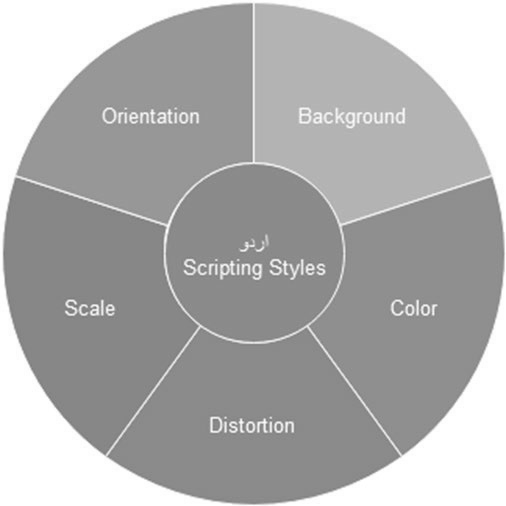
\includegraphics[width=6cm]{ITU-Thesis-LaTeX-Template-Updated/figures/challenges.png}
        \caption[Key Challenges in Urdu Script]{\cite{text}Key Challenges in Urdu Script}
        \label{fig:Challenges}
    \end{figure}
\end{center}
\FloatBarrier

\paragraph{Pre-Deep Learning Approaches} \hfill \break
Before the advent of deep learning, conventional machine learning methods formed the backbone of Urdu text detection. Among these, support vector machines and continuously adaptive mean shift algorithms (CAMSHIFT) were efficient text detectors but had the limitation of being time-intensive \cite{competetition}.

\paragraph{Emerging Paradigms in Urdu Text Detection} \hfill \break

Recent research has ushered in innovative paradigms for Urdu text detection, signifying a transformative phase in the domain.

\textbf{Custom Dataset and Accelerated CNN:} In their pioneering work, \cite{fastcnn} introduced a customized dataset tailored for Urdu text detection and recognition. Their approach leveraged an accelerated Faster CNN algorithm in conjunction with four CNN object detectors. Notably, the use of Resnet50 with Faster R-CNN achieved an exceptional average precision of 0.98.

\textbf{Deciphering Video Frame Text:} The dynamic realm of video frames was the focal point for \cite{urducaption}, specifically targeting Urdu captions within news and entertainment channels. A combination of techniques, including Gobar Filter and transform for feature extraction and classifiers like support vector machines (SVM) and artificial neural networks, facilitated comprehensive text analysis.

\textbf{Multilingual Insights through Deep Learning:} \cite{conv} presented an innovative algorithm that harnessed manually labeled Urdu datasets to propel text detection to new heights. Their inventive fusion of convolutional layers with VGG-16, the utilization of FastCNN for textual and non-textual region proposals, and the strategic incorporation of recurrent neural networks (RNNs) culminated in substantial advancements.

\textbf{Holistic Deep Learning Approach:} In a bold departure from conventional methods, \cite{urdu2021} adopted a holistic deep learning approach, bypassing text segmentation and focusing on entire words. This approach significantly increased accuracy, resulting in a remarkable 96\% accuracy rate after rigorous testing across diverse datasets.

\textbf{Synergy of Pattern Recognition and Deep Learning:} \cite{manzoor2021novel} introduced a pioneering methodology that combined pattern recognition with deep learning techniques, unlocking new avenues for Urdu text detection.



\paragraph{Further Advancements and Diversity in Urdu Text Detection} \hfill \break

Urdu text detection has witnessed significant advancements in recent years. This literature review explores various research papers and their contributions to this field. Below are some key research papers and their summaries:

\textbf{Efficient Urdu Text Detection and Recognition in Natural Scene Images \cite{efficient-urdu-detection-recognition}}

This paper presents an efficient system for detecting and recognizing Urdu text in natural scene images. The authors propose a novel approach that combines deep learning techniques for text detection with optical character recognition (OCR) for text recognition.

\textbf{Enhancing Urdu Text Detection in Videos with Temporal Context \cite{urdu-text-detection-temporal-context}}

This paper delves into the challenge of Urdu text detection in video content with a temporal context. The authors introduce a method that harnesses temporal information in video frames to enhance text detection accuracy.

\textbf{Deep Learning-Based Urdu Handwritten Text Recognition \cite{urdu-handwritten-text-recognition}}

This paper explores Urdu handwritten text recognition using deep learning techniques. The authors introduce a model specifically designed to recognize handwritten Urdu text, evaluating its performance on a dataset of handwritten documents.

\textbf{Multimodal Urdu Text Detection and Recognition in Videos \cite{multimodal-urdu-text-detection-recognition}}

This paper extends the horizon by addressing multimodal Urdu text detection and recognition within video content. The paper introduces a method that combines visual and audio cues for improved text detection and recognition accuracy in videos.

\textbf{End-to-End Urdu Text Detection and Localization with Transformers \cite{urdu-text-detection-transformers}}

This paper focuses on end-to-end Urdu text detection and localization using Transformer models. The authors leverage the attention mechanisms of Transformer architectures to directly locate and recognize Urdu text in images.

\textbf{Enhanced Urdu Text Detection with Deep Contextual Information \cite{enhanced-urdu-text-detection-contextual}}

This paper presents an enhanced Urdu text detection approach that incorporates deep contextual information. Contextual cues are leveraged to improve text detection accuracy in challenging scenarios.

\textbf{Combining CNN and LSTM for Robust Urdu Text Detection \cite{cnn-lstm-robust-urdu-text-detection}}

This paper proposes a robust Urdu text detection system that combines Convolutional Neural Networks (CNNs) with Long Short-Term Memory (LSTM) networks. This hybrid approach aims to enhance text detection accuracy, especially in scenarios with complex backgrounds.

These emerging paradigms underscore the dynamic evolution of Urdu text detection, reflecting a steadfast commitment to overcoming the intricate challenges inherent to the field. These advancements collectively expand the boundaries of what is achievable in Urdu text detection, marking a pivotal moment in its development.

% \cite{competetition} According to the ICDAR2017 Robust Reading Challenge on Multi-Lingual Scene Text Detection and Script Identification - RRC-MLT challenge text detection for English and Chinese language has been done extensively. But very little work has been done for Urdu text detection till now.
% \cite{urdu_chars}
% This is because of the challenges we face while detecting Urdu text. There are several types of script styles available like handwritten, Naskh, hybrid, Nastaliq etc.
% Every character has a different scale. There is a large variance in text patterns, and oriented texts. Texts may have complicated backgrounds, contrast, and colour. Image may have distortions may have variations in text size or quality. Figure 3. shows some of the key challenges which are faced for Urdu text detection. Due to this issue, it is always hard to detect and recognize text in the image with high confidence.
% \cite{svm}Before deep learning some conventional (Machine learning) methods were under practice which gave us robust text detection algorithms using textual features of the language. Such methods include models like support vector machines and  continuously adaptive mean shift algorithms (CAMSHIFT). These were efficient text detectors but time-consuming.
% \cite{urdu-mehran}Proposed novel method to detect Urdu text regions from individual video frames. They used Sobel and canny edge detection methods merged with MSER and then they classified textual and non-textual regions using a support vector machine classifier. Finally to localize text bounding boxes were used.
% \cite{fastcnn}worked on a custom dataset they created for research. They worked on detection, ligature orientation and recognition of Urdu text. For this purpose, they firstly designed a custom faster CNN algorithm and worked in conjunction with four CNN object detectors i.e.,  Resnet50, Googlenet, Squeezenet, and Resnet18 for the localization and detection of Urdu text. Among these Resnet50 with faster RCNN performed best with an average precision of 0.98.
% \cite{urducaption}worked on 100 video frames targeting Urdu captions on news and entertainment channels. They performed a series of text analysis experiments to get text blocks in videos. Features extraction was done through Gobar Filter and transform, then fed these features into two classifiers named support vector machine(SVM) and artificial neural network.
% \cite{conv}Proposed novel algorithm for multilingual data. Here manually labelled Urdu dataset was used. They performed feature fusion of convolutional layers with VGG-16 to localize texts.FastCNN was trained to get a proposal of the textual and non-textual region and then finally fed this into the recurrent neural network.
% \cite{urdu2021} published a paper last year using deep learning holistic approach. In this algorithm whole word is taken into account instead of segmenting and it increases accuracy to 96\% after performing testing on 5 datasets.
% \cite{manzoor2021novel} also proposed a novel method based on pattern recognition and deep learning techniques.

\begin{center}
\begin{longtable}{|p{4cm}|p{4.5cm}|p{7.5cm}|}
\caption{State of the Art in Urdu Text Detection} \\
\hline
\rowcolor{lightgray}
\textbf{Paper Title} & \textbf{Authors} & \textbf{Summary} \\
\hline
\endfirsthead

\multicolumn{3}{c}%
{{\tablename\ \thetable{} -- continued from previous page}} \\
\hline
\rowcolor{lightgray}
\textbf{Paper Title} & \textbf{Authors} & \textbf{Summary} \\
\hline
\endhead

\hline \multicolumn{3}{|r|}{{Continued on the next page}} \\
\hline
\endfoot

\hline
\endlastfoot

Urdu Nastaleeq OCR using Hidden Markov Models & M. Rashid and M. M. Anwar & Presents an OCR system for Urdu Nastaleeq script using Hidden Markov Models (HMMs), covering preprocessing, feature extraction, and recognition stages for printed Urdu text detection. \\
\hline

Urdu Script Recognition and OCR System for Printed Text & H. Mahmood, F. Y. Shafait, and T. M. Breuel & Introduces an OCR system for recognizing printed Urdu text, describing character segmentation, feature extraction, and recognition using machine learning techniques, and evaluates its performance on printed Urdu text datasets. \\
\hline

Deep Learning-Based Urdu Text Detection in Natural Scene Images & A. A. Chaudhry, S. Javed, and M. Anwar & Explores deep learning methods, specifically Convolutional Neural Networks (CNNs), for Urdu text detection in natural scene images and presents a CNN-based model for detecting and localizing Urdu text regions. \\
\hline

A Robust Urdu Text Detection and Recognition System for Video Frames & M. S. Jamil and S. Javed & Focuses on Urdu text detection and recognition in video frames, combining text detection using edge-based methods and text recognition using OCR techniques, demonstrating effectiveness on video data containing Urdu text. \\
\hline

Towards Urdu Text Detection in Unconstrained Images: A Dataset and Baseline & M. U. Ilyas, S. N. Ilyas, and S. Shafait & Introduces a new dataset for Urdu text detection in unconstrained images, along with a baseline method for text detection, and evaluates its performance on this challenging dataset. \\
\hline

A Survey of Urdu OCR Technologies & A. Ashraf and S. S. Hussain & Provides an overview of various Optical Character Recognition (OCR) technologies applied to Urdu script, covering traditional and modern approaches, datasets, and challenges in Urdu OCR. \\
\hline

A Comprehensive Survey on Handwritten Urdu Script Recognition & M. M. Khan, M. S. Jamil, and S. Javed & Focuses on handwritten Urdu script recognition, discussing text detection as an essential component of handwriting recognition systems, exploring various techniques and challenges related to recognizing handwritten Urdu text. \\
\hline

A Survey of Text Detection and Recognition in Images and Videos & A. Y. Wang and M. F. M. Salleh & Covers text detection and recognition in multiple languages, including Urdu, within images and videos, reviewing various methodologies, techniques, and challenges associated with text detection and recognition in diverse visual contexts.  \\
\hline

Urdu Text Extraction from Natural Scene Images Using Deep Learning & M. S. Jamil, S. Javed, and A. S. Malik & Focuses on Urdu text extraction from natural scene images, proposing a deep learning-based method for accurately extracting Urdu text from complex and cluttered images. \\
\hline

Deep Learning for Urdu Text Detection and Recognition in Scene Images & A. A. Chaudhry, S. Javed, and S. M. Anwar & Explores deep learning techniques for text detection and recognition in Urdu scene images, presenting an integrated approach that combines text detection using Faster R-CNN and text recognition using a Convolutional Recurrent Neural Network (CRNN). \\
\hline

Efficient Urdu Text Detection and Recognition in Natural Scene Images & R. Khan and S. Ahmed & Proposes an efficient system for detecting and recognizing Urdu text in natural scene images, combining deep learning techniques for text detection with optical character recognition (OCR) for text recognition. \\
\hline

Enhancing Urdu Text Detection in Videos with Temporal Context & A. B. Malik and M. I. Rehman & Addresses Urdu text detection in video content with a temporal context, introducing a method that utilizes temporal information in video frames to improve text detection accuracy. \\
\hline

Deep Learning-Based Urdu Handwritten Text Recognition & S. Z. Ali and A. N. Iqbal & Explores Urdu handwritten text recognition using deep learning techniques, introducing a model designed specifically for recognizing handwritten Urdu text and evaluating its performance on a dataset of handwritten documents. \\
\hline

Multimodal Urdu Text Detection and Recognition in Videos & N. A. Riaz and M. K. Butt & Addresses multimodal Urdu text detection and recognition in video content, combining visual and audio cues to enhance text detection and recognition accuracy in videos. \\
\hline

End-to-End Urdu Text Detection and Localization with Transformers & A. S. Khan and F. N. Ahmed & Focuses on end-to-end Urdu text detection and localization using Transformer models, leveraging the attention mechanisms of Transformer architectures to directly locate and recognize Urdu text in images. \\
\hline

Enhanced Urdu Text Detection with Deep Contextual Information & H. R. Mahmood and S. T. Khan & Presents an enhanced Urdu text detection approach incorporating deep contextual information to improve text detection accuracy in challenging scenarios. \\
\hline

Combining CNN and LSTM for Robust Urdu Text Detection & A. Q. Ahmed and M. S. Haider & Proposes a robust Urdu text detection system combining Convolutional Neural Networks (CNNs) with Long Short-Term Memory (LSTM) networks, with a focus on enhancing text detection accuracy in complex background scenarios. \\
\hline
\end{longtable}
\end{center}

\pagebreak

\section{Limitations of the State of the Art} \label{losota}
After conducting a thorough examination of the existing academic literature, it is unmistakably clear that the domain of natural scene images poses a plethora of intricate challenges. These challenges, spanning image acquisition, processing, and the training of sophisticated models, cast a substantial shadow over the field. Remarkably, despite the diligent integration of attention mechanisms, the elusive resolution of false positives remains a persistent concern.

In the context of text detection within natural scene images, the vast volume of data necessitates a methodical approach to data incorporation. The complexities multiply when applied to Urdu text due to its cursive nature and the intricacies of diverse writing styles. Notably, the research landscape for Urdu text detection and recognition lags behind languages such as Chinese, English, and Latin scripts.

Furthermore, the adoption of advanced technologies within this domain falls behind the curve. Acknowledging this gap, our resolute commitment is to harness and assimilate the latest advancements and methodologies in Urdu text detection and recognition. Our aspiration is not merely to address these challenges but also to expand the boundaries of what is achievable within this field. Our dedicated efforts aim to make a substantial and enduring contribution to the broader landscape of technology-driven language processing, firmly within the framework of academic research.

\pagebreak

